% pdflatex -shell-escape -interaction=nonstopmode main.tex && pdflatex -shell-escape -interaction=nonstopmode main.tex

\chapter{Grundlagen} \label{basics}

Dieses Kapitel bietet Einblick in die Grundlagen von \textbf{Genetischen Algorithmen} (Kap. \ref{ga-my-definition}) im Zusammenhang mit \textbf{neuronalen Netzen} (Kap. \ref{neural-evo-definition}) und der \textbf{Cross Entropy Method} (Kap. \ref{cross-entropy-definition}). Außerdem werden einige Verbesserungen zu den naiven Methoden besprochen, wie die Reduzierung des Suchraums durch \textbf{Fourier-Transformationen} und die Einführung von einer \textbf{kooperativen Evolution} durch Hinzufügen von einer neuen Aktion zu dem Ablauf des genetischen Algorithmus.

    \section{Genetische Algorithmen} \label{ga-my-definition}
        % ``Die Motivation von Genetischen Algorithmen kam aus der Natur bla blubb''\\
        % ``Im Folgenden behandeln wir die grundlegenden Operationen die einen GA ausmachen''

        % Ein Genetischer Algorithmus gehört zu den \textbf{unsupervised Learning} Methoden, die sich als Ziel setzen eine verborgene Struktur zu analysieren, ohne zu gekenntzeichnete Daten zu haben. John Holland

        Ein genetischer Algorithmus (\textit{genetic algorithm}), im folgenden als \textbf{GA} abgekürzt, ist ein Optimierungsverfahren, das von der natürlichen Selektion und Evolution inspiriert ist. Ein formaler Leitfaden findet sich im Fundamentalwerk zu genetischen Algorithmen \cite{ga}.\\[2mm]
        Stellen wir uns anschaulicher Weise eine Gruppe Gazellen und einen Geparden vor.\\

        \begin{figure}[htbp]
            \begin{subfigure}{0.5\textwidth}
                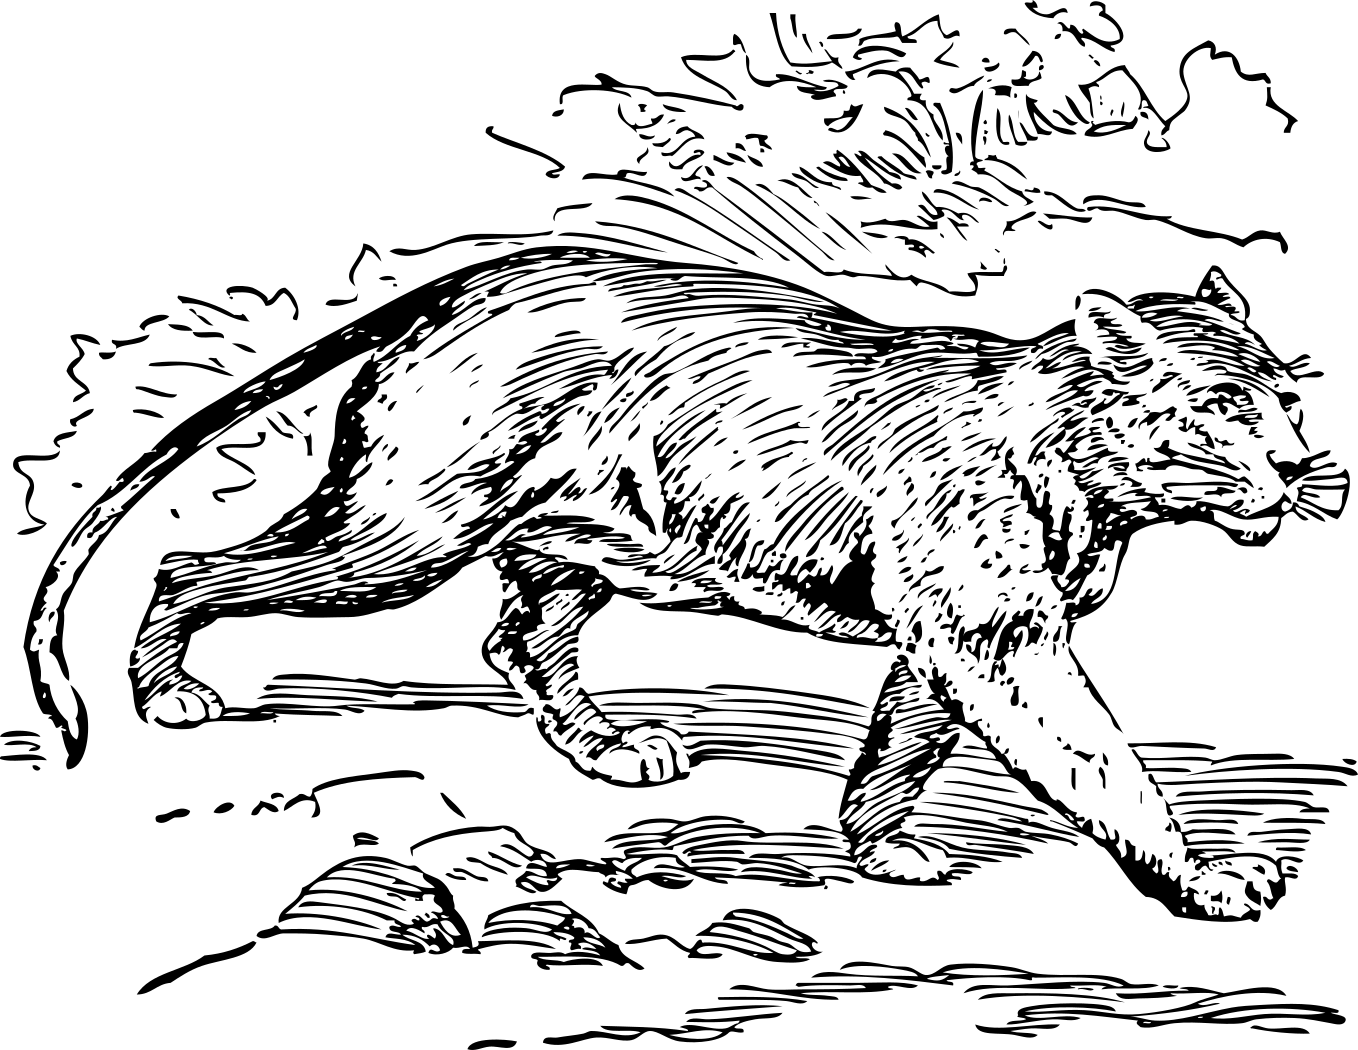
\includegraphics[width = 1\textwidth, left]{../pictures/cheetah.png}
            \end{subfigure}
            \begin{subfigure}{0.5\textwidth}
                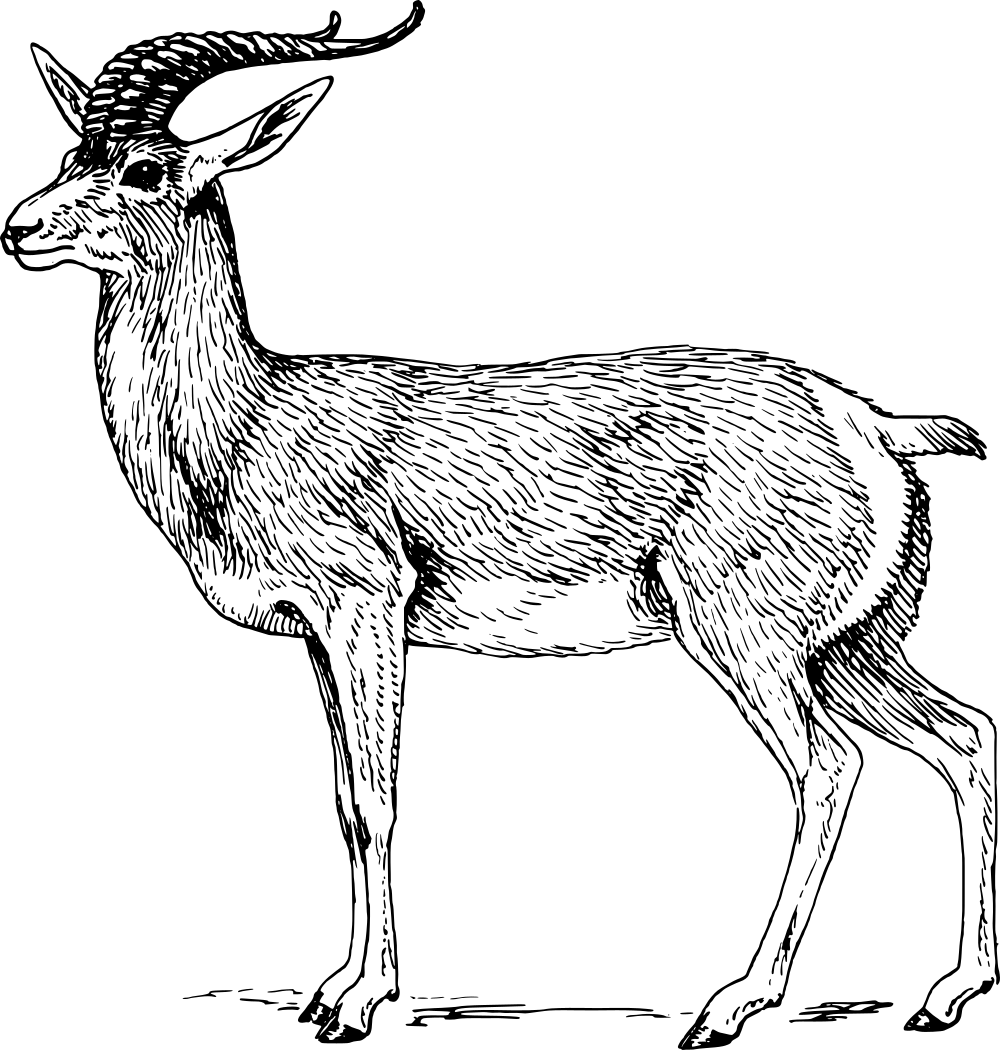
\includegraphics[width = 0.73\textwidth, right]{../pictures/gazelle.png}
            \end{subfigure}
            \caption{Illustration eines Geparden und einer Gazelle \label{fig:gazelleAndGepard}}
        \end{figure}
        \noindent
        Sei unser Gepard durch seine Geschwindigkeit den Gazellen überlegen, dann wird die Gazellenherde über Zeit in ihrer Anzahl sinken. Dabei werden die langsamen Gazellen dem Geparden erliegen und die Schnelleren überleben. Dieser Schritt wird als \textbf{Selektion} bezeichnet. Die Überlebenden werden sich fortpflanzen und mit hoher Wahrscheinlichkeit Gazellen-Babies bekommen die ähnlich schnell sind. Diesen Vorgang bezeichnen wir als \textbf{Kreuzung}. Mit welcher Wahrscheinlichkeit jedes einzelne Tier vor dem Geparden entwischen kann nennen wir \textbf{Fitness}.\\
        \\
        Jede Gazelle, oder auch \textbf{Individuum} genannt, hat eine eigene Fitness, die es aber bei Geburt noch nicht weiß, da sie noch nie vor einem Geparden weglaufen musste. Erst nachdem sie einmal erfolgreich entwischt ist, können wir uns vorstellen, was ihre Fitness ist.\\
        \\
        Ganz selten wird ein Gazellen-Baby geboren, das ein etwas längere Beine hat als alle anderen, dabei hatte keiner dieses Merkmal vor ihr. Das erlaubt ihr schneller zu laufen, was für sie erstmal positiv ist. Diese Ausprägung hat jedoch den Nachteil, dass die Standhaftigkeit darunter leidet. Diese unerwartete Veränderung bei den Kindern heißt \textbf{Mutation}.\\
        \\
        Fassen wir zusammen: Nachdem jede überlebte Gazelle sich fortgepflanzt hat, bekommen wir hoffentlich wieder eine vollzähliges Herde, die wir \textbf{Population} nennen. Nach all diesen Schritten fängt der Kampf um das Überleben wieder an und geht solange, bis sich entweder Gazellen entwickeln, die dem Gepard ständig entkommen können, oder bis die gesamte Population ausstirbt.\\
        \\
        Damit haben wir die wichtigsten Begrifflichkeiten von einem genetischen Algorithmus erklärt und kommen zur Umsetzung der einzelnen Schritte.

        \subsection{Individuen}

            Ein Individuum besteht aus einer Kodierung, auch \textbf{Zustandsraum} genannt, die die aussagekräftigen Eigenschaften von ihm ausmachen. Für eine Gazelle wäre beispielweise die Kodierung aus \ref{tab:gaz-encoding} möglich.

            \begin{multicols}{2}
                \hfill \\[-10mm]
                \begin{table}[H]
                    \begin{center}
                    \begin{tabular}{ |l|r| } 
                        \hline
                        Höchstgeschwindigkeit    & $ 95\; \frac{km}{h}$   \\ \hline
                        Beinlänge                & $ 86\; cm          $   \\ \hline
                        Gewicht                  & $ 43\; kg          $   \\ \hline
                        Hornlänge                & $ 12\; cm          $   \\ \hline
                    \end{tabular}
                    \end{center}
                    \caption{Kodierung einer Gazelle \label{tab:gaz-encoding}}
                \end{table}

                \noindent
                Die Aufgabe von unserem GA ist ein oder mehrere Individuen zu finden, die es schaffen vor dem Geparden wegzulaufen. Da wir aber nicht wissen, ob die vorgeschlagene Kodierung gut oder schlecht ist, müssen wir Gazellen mit zufälligen Eigenschaften erstellen und dann den Algorithmus arbeiten lassen.
            \end{multicols}
            \noindent
            Das schaffen wir, indem wir Grenzen für die Kodierung festlegen (Tabelle \ref{tab:gazelle-bounds}) und später zufällige Werte in diesen Rahmen ausprobieren.

            \begin{table}[H]
                \begin{center}
                \begin{tabular}{ |l|r|r| } 
                    \hline
                    Eigenschaft              & Minimaler Wert        & Maximaler Wert       \\ \hline
                    Höchstgeschwindigkeit    & $ 20\; \frac{km}{h}$  & $ 100\; \frac{km}{h}$ \\ \hline
                    Beinlänge                & $ 40\; cm          $  & $ 90\; cm          $ \\ \hline
                    Gewicht                  & $ 12\; kg          $  & $ 75\; kg          $ \\ \hline
                    Hornlänge                & $  0\; cm          $  & $ 35\; cm          $ \\ \hline
                \end{tabular}
                \end{center}
                \caption{Grenzen für die Kodierung \cite{wiki:gazelle} \cite{blog:gazelle}\label{tab:gazelle-bounds}}
            \end{table}
            \noindent
            % Für die Kodierung unseres Individuums eignet sich ein Array von Zahlen. Um die gesamte Population darzustellen würde ein 2-dimensionales Array reichen, wobei jedes Element ein einzelnes Individuum darstellt. \textit{(evtl Grafik)}

        \subsection{Evaluation}
            Nachdem wir unsere Gazellenpopulation erstellt haben, müssen wir sie der Natur überlassen. Dann ist es unsere Aufgabe nach einer festen Zeitspanne und sie alle wieder aufzusammeln. Dadurch finden wir heraus wie viele Gazellen überlebet haben und können diese Information den nächsten genetischen Methoden übergeben.

        \subsection{Selektion}

            Nachdem die Evaluation vorbei ist, bekommen wir die Rückmeldung welche Gazellen überlebt haben. Aus dieser Menge können wir nun einen prozentualen Betrag wählen, die Eltern sein werden. In unserer Implementierung nennen wir diesen Parameter $\alpha$. Damit versichern wir, dass nur die erfolgreichen Eigenschaften weiter in der Population erhalten bleiben und der Rest wegfällt.

        \subsection{Kreuzung}
            Die erfolgreichen Individuen wurden ausgewählt und können sich nun fortpflanzen. Dafür nehmen wir jeweils zwei Individuen und vertauschen zufällig ihre Ausprägungen. Dieses Verfahren haben wir in den Tabellen \ref{fig:enc-dad}, \ref{fig:enc-mom}, \ref{fig:child-1}, \ref{fig:child-2} dargestellt.
            \\[8mm]
            \begin{multicols}{2}
                \begin{table}[H]
                    \begin{center}
                    \begin{tabular}{ |r| } 
                        \hline
                        \hfill Eigenschaften  \\ \hline
                        \cellcolor{blue!25} $ 56\; \frac{km}{h}$ \\ \hline
                        \cellcolor{blue!25} $ 42\; cm          $ \\ \hline
                        \cellcolor{blue!25} $ 51\; kg          $ \\ \hline
                        \cellcolor{blue!25} $ 10\; cm          $ \\ \hline
                    \end{tabular}
                    \end{center}
                    \caption{Kodierung des Vaters \label{fig:enc-dad}}
                \end{table}

                \begin{table}[H]
                    \begin{center}
                    \begin{tabular}{ |r| } 
                        \hline
                        \hfill Eigenschaften  \\ \hline
                        \cellcolor{yellow!25} $ 62\; \frac{km}{h}$ \\ \hline
                        \cellcolor{yellow!25} $ 55\; cm          $ \\ \hline
                        \cellcolor{yellow!25} $ 49\; kg          $ \\ \hline
                        \cellcolor{yellow!25} $  8\; cm          $ \\ \hline
                    \end{tabular}
                    \end{center}
                    \caption{Kodierung der Mutter \label{fig:enc-mom}}
                \end{table}

            \end{multicols}

            \begin{multicols}{2}
                \begin{table}[H]
                    \begin{center}
                    \begin{tabular}{ |r| } 
                        \hline
                        \hfill Eigenschaften  \\ \hline
                        \cellcolor{blue!25}   $ 56\; \frac{km}{h}$ \\ \hline
                        \cellcolor{yellow!25} $ 55\; cm          $ \\ \hline
                        \cellcolor{yellow!25} $ 49\; kg          $ \\ \hline
                        \cellcolor{blue!25}   $ 10\; cm          $ \\ \hline
                    \end{tabular}
                    \end{center}
                    \caption{Kodierung vom Kind Nr.1 \label{fig:child-1}}
                \end{table}


                \begin{table}[H]
                    \begin{center}
                    \begin{tabular}{ |r| } 
                        \hline
                        \hfill Eigenschaften  \\ \hline
                        \cellcolor{yellow!25} $ 62\; \frac{km}{h}$ \\ \hline
                        \cellcolor{blue!25}   $ 42\; cm          $ \\ \hline
                        \cellcolor{blue!25}   $ 51\; kg          $ \\ \hline
                        \cellcolor{yellow!25} $  8\; cm          $ \\ \hline
                    \end{tabular}
                    \end{center}
                    \caption{Kodierung vom Kind Nr.2 \label{fig:child-2}}
                \end{table}
            \end{multicols}
            \noindent
            Das können wir nun sooft wiederholen, wie wir Eltern finden, oder bis wir genug Kinder produziert haben.

            \newpage
            In unserem Beispiel haben wir die Kinder mit dem folgenden Python-Code konstruiert:
            \hfill \\
            \begin{mdframed}
            \begin{minted}[escapeinside=||, linenos]{python}
vater  = [56,42,51,10]
mutter = [62,55,49,8]
kind1  = []
kind2  = []
for i in range(kodierung.length):
    r = random.uniform(0,1)
    if (r > 0.5):
        kind1[i] = vater[i]
        kind2[i] = mutter[i]
    else:
        kind1[i] = mutter[i]
        kind2[i] = vater[i]
            \end{minted}
            \end{mdframed}
            \hfill \\[4mm]
            \noindent
            In \textit{Z.1-2} definieren wir die Eigenschaften der Mutter und des Vaters. Dann iterieren wir durch die Länge der Kodierung (\textit{Z.5}) und wählen mit einer 50\% Wahrscheinlichkeit (\textit{Z.6-7}) aus für jedes Kind aus, ob die gewählte Eigenschaft vom Vater oder von der Mutter kommt.\\

            \noindent
            Diese Art und Weise zwei Individuen zu kreuzen nennt sich \textbf{n-point crossover}, weil wir die Kodierung an zufällig vielen Stellen unterbrechen. Es gibt noch andere Kreuzungsmethoden die eine eine feste Anzahl von Aufteilungen benutzen, wie \textbf{one-} oder \textbf{two-point crossover}. \\
            \\
            \noindent
            Um einen Unterschied zwischen diesen Methoden zu erkennen, stellen wir uns vor dass die Beinlänge im Zusammenhang mit der Höchstgeschwindigkeit steht, weil längere Beine eine größere Sprungweite ermöglichen. Wenn nun ein Kind gezeugt wird, dass lange Beine vererbt, wird die Höchstgeschwindigkeit dadurch nicht automatisch angepasst. Deshalb wäre es besser, wenn diese Ausprägungen zusammen übernommen werden, weil dadurch eine höhere Fitness garantiert werden kann. Kreuzungsmethoden wie \textit{n-point crossover} verletzen diese Eigenschaft eher als wie \textit{one-point crossover}.\\
            \\
            \noindent
            Je nach Implementierung verwendet man nur eins der beiden Kinder, weil das die Varianz der Gesamtpopulation weniger beeinflusst und trotzdem keinerlei Information verloren geht, weil die Eltern die Kodierung weiter tragen.

\newpage
        \subsection{Mutation}
%            ``Mutation ist hilfreich um die Varianz der Population etwas zu erhöhen'' \\
            Nachdem die Kinder erstellt wurden, müssen wir die Kodierung der Individuen etwas verändern, damit die Varianz in der Gesamtpopulation erhöht wird. Das machen wir indem wir durch die Kodierung der Kinder durchgehen und jede Ausprägung mit einer geringen Wahrscheinlichkeit verändern. Diese nennen wir $\beta$. Die Tabellen \ref{fig:child-enc} und \ref{fig:mut-child-enc} zeigen diese Veränderung am Beispiel des Kindes aus Tabelle \ref{fig:child-2}.

            \hspace*{-2cm}
            \begin{multicols}{2}
                \begin{table}[H]
                    \begin{center}
                    \begin{tabular}{ |r| } 
                        \hline
                        \hfill Eigenschaften  \\ \hline
                        \cellcolor{yellow!25} $ 62\; \frac{km}{h}$ \\ \hline
                        \cellcolor{blue!25}   $ 42\; cm          $ \\ \hline
                        \cellcolor{blue!25}   $ 51\; kg          $ \\ \hline
                        \cellcolor{yellow!25} $  8\; cm          $ \\ \hline
                    \end{tabular}
                    \end{center}
                    \caption{Kodierung von einem Kind \label{fig:child-enc}}
                \end{table}

                \begin{table}[H]
                    \begin{center}
                    \begin{tabular}{ |r| } 
                        \hline
                        \hfill Eigenschaften  \\ \hline
                        \cellcolor{yellow!25} $ 62\; \frac{km}{h}$ \\ \hline
                        \cellcolor{blue!25}   $ 42\; cm          $ \\ \hline
                        \cellcolor{red!25}    $ 45\; kg          $ \\ \hline
                        \cellcolor{yellow!25} $  8\; cm          $ \\ \hline
                    \end{tabular}
                    \end{center}
                    \caption{Mutierte Kodierung vom Kind\label{fig:mut-child-enc}}
                \end{table}
            \end{multicols}

            Die Mutation kann folgendermaßen in Python umgesetzt werden:
            \begin{mdframed}
            \begin{minted}[escapeinside=||, linenos]{python}
kinder = [k1, k2...]
beta   = 0.1
for i in range(kinder.length):
    for j in range(kodierung.length):
        r = random.uniform(0,1)
        if (r > beta):
            kinder[i][j] = sampleNewFrom(kodierung[j].range)
            \end{minted}
            \end{mdframed}
            \hfill \\[1mm]
            \noindent
            In \textit{Z.1-2} definieren wir Mutationswahrscheinlichkeit und die Kinder. Dann gehen wir jede Kodierung von jedem Kind durch (\textit{Z.3-4}) und verändern die Eigenschaft mit einer 10\% Wahrscheinlichkeit (\textit{Z.5-7}).\\

            \noindent
            Dieser Schritt ist wichtig, sodass trotz konvergierter Population neue Eigenschaften ausprobiert werden, da sie vielleicht eine bessere Lösung bieten. Der GA tendiert oft dazu sich erstmal für eine suboptimalen Lösung zu entscheiden und die Mutation erlaubt uns einen Ausweg daraus. \\

            \noindent
            In manchen Fällen kann man die Mutation noch weiter parametrisieren, indem man ein Veränderungsfaktor als Argument hinzufügt. Diese Technik benutzt man, wenn die Kodierung nicht trivialerweise verändert werden kann, da sonst bestimmte Eigenschaften verloren gehen. In Kapitel 3 wird genau so ein Fall besprochen, weil wir unsere Individuen durch eine Wahrscheinlichkeitsverteilung darstellen. 

\newpage

        \subsection{Repopulation}
            Die Eltern wurden ausgewählt, die Kindern gezeugt und mutiert, nun müssen wir die Population in eine Form bringen, sodass die Evaluation neu gestartet werden kann. Wir stellen das Problem wieder an einem Beispiel dar.\\

            \begin{mdframed}
            \begin{minted}[escapeinside=||, linenos]{python}

population = [i1,i2,...]                  # population.length = 10
alpha      = 0.4
eltern     = selection(population, alpha) # eltern.length = 4
kinder     = crossover(eltern)            # kinder.length = 4
beta       = 0.1
mutkinder  = mutation(kinder, beta)       # mutkinder.length = 4

newpopulation = eltern + mutkinder        # newpopulation.length = 8
            \end{minted}
            \end{mdframed}
            \hfill \\
            \noindent
            Wir sehen, dass in der neuen Population zwei Individuen fehlen und können die Simulation deshalb nicht neu starten. Dieses Problem kann man auf viele Weisen angehen, die ihre eigenen Vorteile und Nachteile haben. 

            \subsubsection*{Mehr Kinder erstellen}
                Es ist möglich während der Kreuzung solange Kinder zu erzeugen, bis die Population wieder ihre Ausgangsgröße angenommen hat. Ein Vorteil wäre, dass diese Individuen mit wahrscheinlich besseren Ausgangskodierungen starten als Neue. Der Nachteil ist jedoch die gesenkte Varianz in der Population und die erhöhte Wahrscheinlichkeit zum Feststecken in einem suboptimalen Lösungen.

            \subsubsection*{Nicht selektiere Individuen nachfüllen}
                Man kann die nicht benutzen Individuen aus der vorherigen Population zum Auffüllen benutzen, was sich aber nur dann gewählt werden sollte, wenn die Chance bestünde, dass sie in der erneuten Simulation besser abschneiden als bisher. Ansonsten nehmen sie den Platz für ein potenziell besseres Individuum weg.

            \subsubsection*{Neue Individuen erstellen}
                In unserer Implementierung haben wir uns für das Nachfüllen von völlig neuen Individuen entschieden, da dadurch die Varianz der Population angehoben wird und dadurch mehr Lösungen möglich sind. Ein Nachteil ist dabei sind die potenziellen Kinder die  keinen Platz bekommen, aber da dadurch keine Information verloren geht, können wir es vernachlässigen.
\newpage

    \section{Neuroevolution} \label{neural-evo-definition}
%        ``Neuroevolution beschäftigt sich mit der Verknüpfung von Genetischen Algorithmen und Neuronalen Netzn''
        Der Begriff der Neuroevolution wurde im Jahre 1988 von D. Whiteley \cite{whiteley88} als alternative Möglichkeit zum Trainieren von künstlichen neuronalen Netzen (\textit{artificial neural network}, \textbf{ANNs}) vorgeschlagen. Dabei wird versucht aus der Synergie von dem \textbf{selbstlernenden Charakter} von ANNs und der \textbf{explorativen Suche} eines GAs eine Taktik oder ein Klassifikator zu entwickeln der völlig neue Lösungen finden kann. Den Beweis dafür hat man bereits im Jahr 1995 am Spiel \textit{Othello} gebracht \cite{othello95}. \\[2mm]
        \noindent
        Wir versuchen in diesem Kapitel einen groben Überblick über die Funktionsweise von ANNs zu verschaffen und stellen den Bezug zu genetischen Algorithmen dar. Eine weitaus formalere Erklärung findet sich im Paper von Derrick H. Nguyen und Berndard Widrow \cite{neuralnetwork-overview}.

        \subsection{Künstliche neuronale Netze}

            Die Idee hinter künstlichen neuronalen Netzen ist der Versuch die Struktur vom menschliche Gehirn nachzuahmen. Ein übliches ANN besteht jedoch aus vielfach weniger Neuronen, meist hundert bis mehrere tausend, wobei unser Gehirn 86 Milliarden\cite{brainsize} besitzt.\\
            \noindent
            Ein künstliches Neuron kann man sich anschaulich als eine Formel vorstellen, die \textbf{eins oder mehrere Eingabesignale} über \textbf{gewichtete Pfade} bekommt, sie \textbf{aufsummiert} und eine \textbf{Aktivierungsfunktion} auf das Ergebnis anwendet, die es auf den Bereich $[0,\infty]$, $[0,1]$, oder $[-1,1]$ abbildet. Dieses Resultat nennen wir $\hat{y}$:

            \begin{figure}[H]
                \begin{mdframed}
                    \noindent
                    Sei $n$ die Anzahl der Eingaben,\\
                    \hspace*{4.5mm}    $X = \{x_1,x_2,...,x_n\}$ ein Vektor der Eingabesignale,\\
                    \hspace*{4.5mm}    $W = \{w_1,w_2,...,w_n\}$ ein Vektor der jeweiligen Gewichte, \\
                    \hspace*{4.5mm}    $\sigma(x) = max(x,0)$ die Aktivierungsfunktion:\\[4mm]
                    \hspace*{50mm} \Resize{4.5cm}{$\widehat{y} = \sigma(\sum^{n}_{i = 1} x_i \cdot w_i)$}
                \end{mdframed}
                \formforfigure
                \caption{\label{neuron-math} Formel zur Berechnung der Ausgabe eines Neurons}
            \end{figure}

            \noindent
            Wenn man nun mehrere von diesen Neuronen in Reihe zusammenschaltet (Abbildung \ref{fig:nntikz}), kriegt man ein vollständig vermaschtes Netz, welches grundsätzlich in drei Schichten unterteilt werden kann:
            \begin{itemize}
                \setlength{\itemsep}{5pt}
                \item \textbf{Eingabeschicht} \\
                    Hier kommt der Ausgangszustand rein, sei es ein kodierter Zustand eines Spiels, RGB Werte von einem Bild, oder der DAX.
                \item \textbf{Versteckte Schicht(en)} \\
                    Dieser Teil des Netzes besteht oft aus mehreren Schichten, da er für die Abstraktion und die Lernfähigkeit verantwortlich ist \cite{ANNModeling}. Er bekommt die Signale aus der Eingabeschicht, die er verarbeitet und weiterleitet.
                \item \textbf{Ausgabeschicht} \\
                    Die Ausgabeschicht ist zum Sammeln der Signale von der vorherigen Schicht zuständig und auf ihren Ergebnissen wird dann eine \textbf{Aktivierungsfunktion} angewendet, die die kumulierten Resultate in eine passende Form bringt. Sie varrieren zwischen einfachen Ja/Nein Aussagen, oder wie wir später kennen lernen werden, auch Wahrscheinlichkeitsverteilungen.

            \end{itemize}

            \tikzset{%
              input neuron/.style={
                circle,
                draw,
                minimum size=1cm,
                fill=inputnode
              },
              hidden neuron/.style={
                circle,
                draw,
                minimum size=1cm,
                fill=hiddennode
              },
              output neuron/.style={
                circle,
                draw,
                minimum size=1cm,
                fill=outputnode
              },
              neuron missing/.style={
                draw=none, 
                scale=1.97,
                text height=0.333cm,
                execute at begin node=\color{black}$\vdots$,
                fill=missingnode
              },
              perceptron/.style={
                circle,
                draw,
                scale=3,
                minimum size=1cm,
                fill=perceptronnode
              }
            }

            \begin{figure}[H]
            \centering
                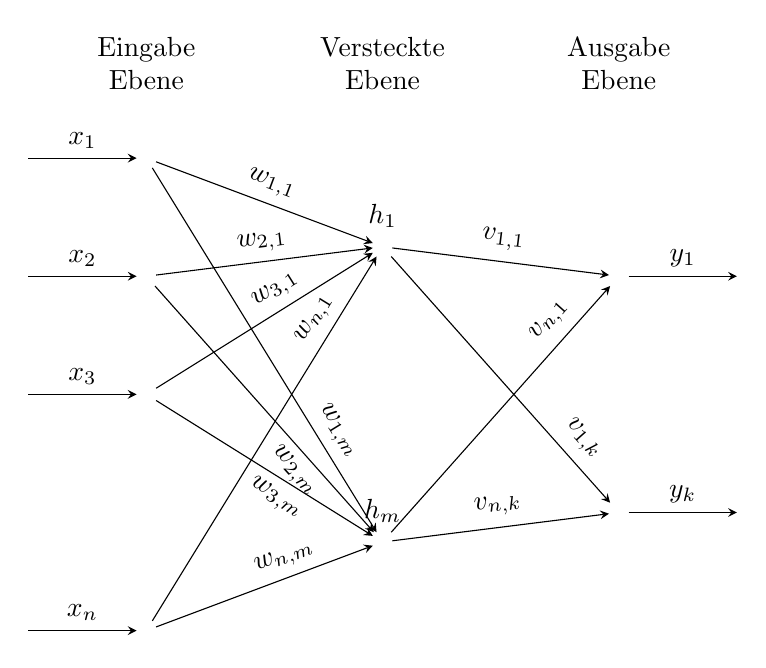
\begin{tikzpicture}[x=1.5cm, y=1.5cm, >=stealth]
                    \foreach \m/\l [count=\y] in {1,2,3,missing,4}
                        \node [input neuron/.try, neuron \m/.try] (input-\m) at (0,2.5-\y) {};
                    \foreach \m [count=\y] in {1,missing,2}
                        \node [hidden neuron/.try, neuron \m/.try ] (hidden-\m) at (2,2-\y*1.25) {};
                    \foreach \m [count=\y] in {1,missing,2}
                        \node [output neuron/.try, neuron \m/.try ] (output-\m) at (4,1.5-\y) {};
                    \foreach \l [count=\i] in {1,2,3,n}
                        \draw [<-] (input-\i) -- ++(-1,0)
                            node [above, midway] {$x_\l$};
                    \foreach \l [count=\i] in {1,m}
                        \node [above] at (hidden-\i.north) {$h_\l$};
                    \foreach \l [count=\i] in {1,k}
                        \draw [->] (output-\i) -- ++(1,0)
                            node [above, midway] {$y_\l$};
%                    \foreach \i [count=\n] in {1,...,4}
%                        \foreach \j [count=\m] in {1,...,2}
%                            \draw [->] (input-\i) -- node [sloped, above, near start] {$w_{\n,\m}$} (hidden-\j); 

                    \draw [->] (input-1) -- node [sloped, above]           {$w_{1,1}$} (hidden-1);
                    \draw [->] (input-1) -- node [sloped, above, near end] {$w_{1,m}$} (hidden-2);

                    \draw [->] (input-2) -- node [sloped, above] {$w_{2,1}$} (hidden-1);
                    \draw [->] (input-2) -- node [sloped, below, pos=0.7] {$w_{2,m}$} (hidden-2);

                    \draw [->] (input-3) -- node [sloped, above, pos=0.6] {$w_{3,1}$} (hidden-1);
                    \draw [->] (input-3) -- node [sloped, below, pos=0.6] {$w_{3,m}$} (hidden-2);

                    \draw [->] (input-4) -- node [sloped, above, pos=0.8] {$w_{n,1}$} (hidden-1);
                    \draw [->] (input-4) -- node [sloped, above, pos=0.625] {$w_{n,m}$} (hidden-2);

%                    \foreach \i [count=\n] in {1,2}
%                        \foreach \j [count=\m] in {1,2}
%                            \draw [line width = 0.0mm, ->] (hidden-\i) -- node [midway, sloped, above=0.3mm] {$v_{\n, \m}$} (
%                            output-\j);

                \draw [->] (hidden-1) -- node [midway, sloped, above=0.3mm] {$v_{1, 1}$} (output-1);
                \draw [->] (hidden-1) -- node [midway, sloped, above=0.3mm, pos=0.8] {$v_{1, k}$} (output-2);
                \draw [->] (hidden-2) -- node [midway, sloped, above=0.3mm, pos=0.8] {$v_{n, 1}$} (output-1);
                \draw [->] (hidden-2) -- node [midway, sloped, above=0.3mm] {$v_{n, k}$} (output-2);

                    \foreach \l [count=\x from 0] in {Eingabe, Versteckte, Ausgabe}
                        \node [align=center, above] at (\x*2,2) {\l \\ Ebene};
                \end{tikzpicture}
                \caption{Skizze von einem vollständig vermaschten künstlichen neuronales Netz \label{fig:nntikz}}
            \end{figure}
            \noindent
            Neuronen wie in Abbildung \ref{fig:nntikz} zusammen zu verknüpfen nennt sich ein \textbf{feedforward} Netzwerk, da es keine Zyklen beinhaltet. Sie besitzen die Einschränkung, dass sie ohne Rücksicht auf die resultierenden Effekte in der Domäne ein Ergebnis liefern, da sie das Signal nur nach vorne weiterleiten.\\

            \noindent
            Um eigene Resultate und zeitliche Abstraktionen zu berücksichtigen gibt es \textbf{rekurrente Netze} die direkte Zyklen beinhalten.

            \subsubsection*{LSTM Ebene} \label{lstm-definition}
                Ein spezielles Neuron aus dem rekurrente Netze bestehen können, ist das \textbf{Long Short Term Memory} (LSTM) Neuron \cite{lstm}. Es zeichnet sich durch die Eigenschaft aus, dass es über lange Zeitfenster Information behalten kann. Der Aufbau basiert auf dem Modell einer Speicherzelle, so dass wir durch verschiedene Eingänge (\textbf{Gates}), die Schreib-, Lese- und Reset-Aktionen nachbauen können \cite{lstm-new}. Einer der wichtigste Aspekte von diesen Neuronen ist jedoch, dass sie ableitbar sind, weil dadurch die Trainingsmethode \textbf{Backpropagation} aus Kapitel \ref{backprop-chapter} ermöglicht wird \cite{backprop}.

            \subsubsection*{Softmax Ebene} \label{softmax-definition}
                Es gibt eine Aktivierungsfunktion der wir besondere Aufmerksamkeit widmen, da sie die Neuronen der Ausgabeschicht zu einem nützlichen Ergebnis zusammenfassen kann. Die generalisierte logistische Funktion (\ref{softmax}), oder auch \textbf{normalisierte Exponentialfunktion} nimmt als Argument einen $k$-dimensionalen Vektor \textbf{z} von reelen Zahlen und gibt uns diesen wieder normalisiert zurück, das bedeutet dass alle Werte auf den Bereich [0,1] gebracht wurden.

            \begin{figure}[H]
                \begin{mdframed}
                    Sei $j = 1,2,...,K$: \\
                    \hspace*{45mm} \Resize{4cm}{$\sigma(\textbf{z})_j = \frac{e^{\textbf{z}_j}}{\sum^{K}_{k = 1} e^{\textbf{z}_k}}$}
                \end{mdframed}
\formforfigure
                \caption{\label{softmax} Definition der Softmax Funktion \cite{softmax-lit}}
            \end{figure}

            \noindent
            Wir könnten argumentieren, dass man für die Normalisierung die Exponentialfunktion nicht benutzen muss. Wenn wir aber als Aktivierungsfunktion die \textbf{Sigmoid Funktion} (\ref{sigmoid}) und als Kostenfunktion den \textbf{logistic loss} oder \textbf{cross entropy loss} benutzt, kürzt sich das $e$ beim im \textit{Backpropagation} Schritt beim partiellen Ableiten weg.

            \begin{figure}[H]
                \begin{mdframed}
                    Sei $t \in \mathbb{R}$:\\
                    \hspace*{50mm} \Resize{3cm}{$S(t) = \frac{1}{1+e^{-t}}$ }
                \end{mdframed}
\formforfigure
                \caption{\label{sigmoid} Definition der Sigmoid Funktion}
            \end{figure}


            \subsection{Backpropagation} \label{backprop-chapter}
                Um diese Technik zum Trainieren von ANNs zu erklären, müssen wir zunächst zeigen wie man den Fehler von einem neuronalen Netz misst. Dafür brauchen wir eine \textbf{Kostenfunktion} die uns die Abweichung zum Soll-Ergebnis gibt. Die Ergebnisse des Netzes für $\widehat{y}$ sind in Abbildung \ref{neuron-math} definiert.

                \begin{figure}[H]
                    \begin{mdframed}
                        \noindent
                        Sei $m$ die Größe des Trainingssets,\\
                        \hspace*{4.5mm} $Y = \{y_0, y_1,\dotsc,y_m\}$ ein Vektor von Soll-Ergebnissen, \\
                        \hspace*{4.5mm} $\widehat{Y} = \{\widehat{y}_0, \widehat{y}_1,\dotsc,\widehat{y}_m\}$ ein Vektor von Resultaten des ANNs, dann ist\\[4mm]
                        \hspace*{30mm} \Resize{7cm}{cost$(Y, \widehat{Y}) = \frac{1}{m} \cdot \sum_{j = 0}^{m} \; (y_j - \widehat{y}_j)^2$}\\[4mm]
                        die mittlere quadratische Abweichung.
                    \end{mdframed}
                    \formforfigure
                    \caption{\label{cost-math}Berechnung des \textit{MSE} Fehlers von einem ANN}
                \end{figure}
                \noindent
                Eine der möglichen Kostenfunktionen sieht man in Formel \ref{cost-math}, die \textbf{mittlere quadratische Abweichung} (\textit{mean squared error}, MSE). Je kleiner das Ergebnis dieser Kostenfunktion ist, umso besser kann unser ANN die Ergebnisse nachahmen. Um die Kosten für eine bestimmte Eingabe zu minimieren, müssen wir herausfinden welche Gewichte aus dem Netz den größten Einfluss hatten und diese entsprechend anpassen. \\

                \noindent
                Anders gesagt, müssen wir den negativen Gradienten der Kostenfunktion entlang wandern. Um ihn zu berechnen, sehen wir in \ref{neuron-math} und \ref{fig:nntikz}, dass die einzigen Faktoren, die das Ergebnis beeinflussen, die Gewichte $(w_1, \dotsc , w_n)$ sind, weil die Eingaben $(x_1, \dotsc , x_n)$ damit multipliziert und aufsummiert werden. Die Aktivierungsfunktion bildet diese Summe lediglich in einen beschränktes Subset der reellen Zahlen ab. \\

                \noindent
                Um ein Netz für bestimme $(x_1, \dotsc , x_n)$ zu trainieren, rechnen wir die jeweilige Vorraussage $\; \widehat{y} = \sigma(\sum^{n}_{i = 1} w_i \cdot x_i) \;$ aus und setzen es in die Kostenfunktion ein. Da wir nur ein einziges Ergebnis haben, wird in der Kostenfunktion die Differenz zum Sollergebnis $y$ berechnet und quadriert, $\; \text{cost}(y, \widehat{y}) = (y - \widehat{y})^2 \;$. \\

                \noindent
                Wenn der berechnete Fehler groß ist, können wir diese Funktion partiell nach dem Gewicht $w_i$ ableiten, um aus dem Gradienten eine \textbf{Anpassungsregel} herzuleiten. Wenn wir auf jedes Gewicht diese Regel, die von dieser bestimmten Eingabe abhängig ist, anwenden, wird der Einfluss derart verändert, dass sie den Fehler den Kostenfunktion minimieren.

                \begin{figure}[H]
                    \begin{mdframed}
                        \noindent
                        Sei $\widehat{y}$ definiert als Ergebnis des Netzes aus \ref{neuron-math}, dann gilt \\
                        pro Beobachtung $\widehat{y}_j \in \widehat{Y}$ und erwartetes Ergebnis $y_j \in Y$, \\
                        leiten wir nach dem Gewicht $w_i$ ab:\\[4mm]
    \hspace*{40mm} \Resize{5.5cm}{$\frac{\partial \text{cost}(y_j,\widehat{y}_j)}{\partial w_i} = \frac{\partial}{\partial w_i} (y_j - \widehat{y}_j)^2$} \\[2mm]
    \hspace*{62.3mm} \Resize{7.0cm}{$ = \frac{\partial}{\partial w_i} (y_j - max(\sum_{i = 0}^{n} x_i \cdot w_i ,0))^2$} \\[2mm]
    \hspace*{62.3mm} \Resize{6.25cm}{$ = -2 \cdot \frac{\partial}{\partial w_i} \; max(\sum_{i = 0}^{n} x_i \cdot w_i ,0)$} \\[2mm]
    \hspace*{62.3mm} \Resize{6.25cm}{$ =   \begin{cases}
                                            0            & \text{ falls }\sum_{i = 0}^{n} x_i \cdot w_i < 0 \\[2mm]
                                            -2 \cdot x_i & \text{ falls }\sum_{i = 0}^{n} x_i \cdot w_i > 0 \\
                                        \end{cases}$}\\[4mm]
                        Damit bekommen wir für Anpassungsregel für jedes Gewicht:\\[4mm]
                        \hspace*{40mm} \Resize{7.5cm}{$w_i \leftarrow w_i + \begin{cases}
                                                                               0 & \text{ falls }\sum_{i = 0}^{n} x_i \cdot w_i < 0 \\[2mm]
                                                                               -2 \cdot x_i & \text{ falls }\sum_{i = 0}^{n} x_i \cdot w_i > 0 \\
                                                                             \end{cases}$}
                    \end{mdframed}
                    \formforfigure
                    \caption{\label{derivative} Beispielhafte Berechnung der Anpassungsregel für $w_i$ nach MSE}
                \end{figure}


            \noindent
            Mithilfe der Anpassungsregel aus \ref{derivative}, die zum alten Gewicht die partielle Ableitung addiert, können wir jedes Mal, wenn das Ergebnis des ANNs zu stark vom Sollergebnis abweicht, diese Regel auf jedes Gewicht anwenden. Damit werden wir uns immer einem Extrema der Kostenfunktion annähern und diese Methode nennt sich \textbf{Fermat's Theorem zu Kritischen Punkten} \cite{miller2009fermat}.\\

            \noindent
            Für unser einfaches Beispiel ist es wahrscheinlich, dass nach dem Anpassen der Gewichte unser ANN das spezifisches Sollergebnis besser erreicht. Damit wird der Fehler reduziert und wir können mit der nächsten Eingaben weitermachen. \\

            \noindent
            Leider haben wir noch ein paar Feinheiten aus dem Fokus gelassen, die sich den Mantelbegriff \textbf{Regularisierung} teilen. Eins der Probleme die Regularisierung löst, passiert wenn unser ANN sich zu stark auf die Trainingsdaten festlegt, aber in der echten Anwendung extreme Abweichungen besitzt. Um das sogenannte \textbf{Overfitting} zu verhindern, gibt es verschiedene Techniken, wie die Anpassung der Lernrate, \textit{weight decay}, \textit{stopped training} oder \textit{noisy data}. Andere Problematiken die bei Backpropagation entstehen und genauere Erklärungen sind im Vorlesungsskript von Machine Learning and Data Mining (2015) von Prof. Dr. Volker Tresp \cite{ml-script} zu finden.\\

            \noindent
            Wenn man auf diese Nuancen achtet, bietet Backpropagation ein extrem mächtiges Instrument, das solange einsetzbar ist, wie das gesamte Netz als Formel dargestellt werden kann, ableitbar ist und damit einen Gradienten liefert an dem wir entlang optimieren können. \\ %Trainingsset an Daten haben.\\

            \noindent
            Unglücklicherweise bieten viele Probleme keine Möglichkeit Trainingsdaten zu sammeln, da das erwünschte Ergebnis keine Rückschlüsse auf den Lösungsweg erlaubt. Anders gesagt, die Kostenfunktion hat keinen Gradienten, den wir verfolgen können. \\ 

            \noindent
            In der Anwendung in der Fußballdomäne aus Kap. \ref{hfo-definition} ist das erwünschte Ergebnis ein Tor, dabei gibt es uns keine Aussage über die notwendigen Schritte. Dieses Fitnesssignal ist so zustandsunabhängig, dass wir nicht einmal wissen, wie viele Spieler auf dem Feld stehen oder ob sie zusammen spielen. Deshalb nutzen wir diese Trainingsmethode lediglich als vergleichendes Beispiel, um ein alternative Methode vorzuschlagen, die trotz dieser Einschränkung lernende Merkmale aufzeigt (\ref{fig:graph-ne}).

        \subsection{Verbindung mit genetischen Algorithmen}
            Wenn wir nun zum Trainieren von ANNs einen genetischen Algorithmus benutzen wollen, müssen wir das Netz als Liste von Gewichten kodieren, aus denen es besteht. Ein Beispiel dafür bietet der \textbf{GENITOR} \cite{moriarty1999evolutionary} Algorithmus (1998). Dabei werden die einzelnen Gewichte der Kreuzung und einer speziellen Mutation ausgesetzt, die von der Varianz der Gesamtpopulation abhängt. \\

            \noindent
            Ein weiterer Ansatz ist \textbf{SANE} \cite{moriarty1999evolutionary} (1999), der gesamte Neuronen für die \textit{Hidden Ebene} entwickelt und gleichzeitig die Netztopologie verändert. Damit versucht es sich an die Komplexität der Aufgabe anzupassen. \\ % Dadurch wurde eine nicht triviale Strategie für das Spiel Othello wiederentdeckt \cite{othello95}. \\

            \noindent
            Problematischerweise benutzen neuronale Netze heutzutage je nach Anwendungsgebiet immer aufwendigere Strukturen, die extrem viele Gewichte besitzen. Eine naive genetische Suche in so einem hochdimensionalen Zustandsraum dauert zu lange und deshalb untersuchen wir Techniken, die uns erlauben zielsicherer und effizienter den Raum aller Möglichkeiten zu durchsuchen. 

\newpage

    \section{Diskrete Kosinustransformation} \label{dct-definition}

        Eine Technik zum reduzieren des Suchraums ist die diskrete Kosinustransformation (\textit{discrete cosine transform}, \textbf{DCT}), die zur Familie der Fourier-Transformationen gehört. Eine \textbf{Fourier-Transformation} teilt ein Signal in beliebig viele trigonometrische Funktionen, wie Sinus oder Kosinus auf, und über die Summe dieser Funktionen kann jedes Signal beschrieben werden. \\

        \noindent
        Diese Fourier-Transformation liefert uns ein diskretes Frenquenzenspektrum, das in Form von Koeffizienten dargestellt wird. Dabei wird pro kodierten Datenpunkt ein Koeffizient erzeugt. Um die Daten wiederherzustellen gibt es die inverse Kosinustransformation, die die Koeffizienten wieder umwandelt.

        \begin{multicols}{2}
            \begin{figure}[H]
                \begin{center}
%                    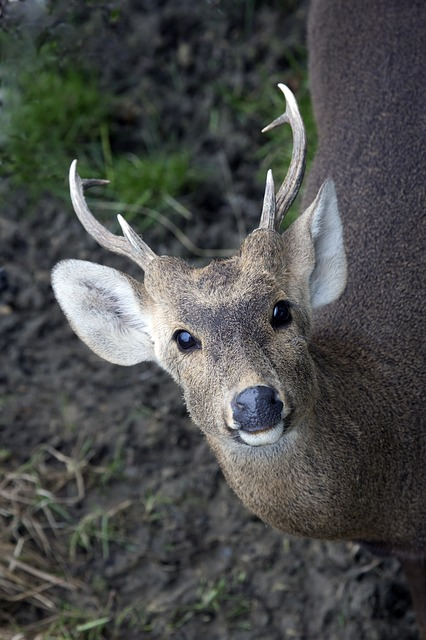
\includegraphics[scale=1]{../pictures/gazelle-uncompressed.jpg}\\
                    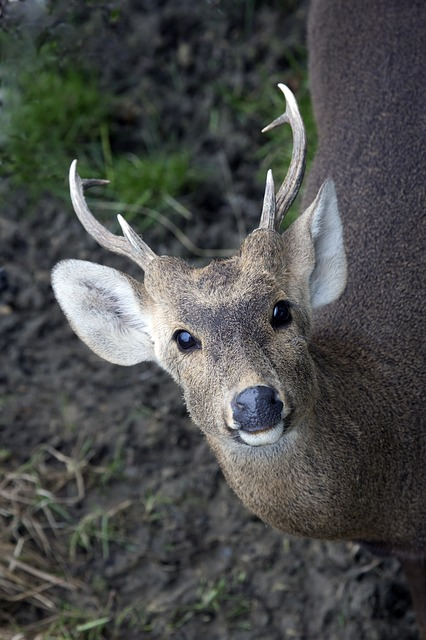
\includegraphics[scale=1.5]{../pictures/gazelle-uncompressed.jpg}\\
                    \caption{Unkomprimiert}\label{fig:gazelle-uncompressed}
                \end{center}
            \end{figure}
            \par
            \begin{figure}[H]
                \begin{center}
                    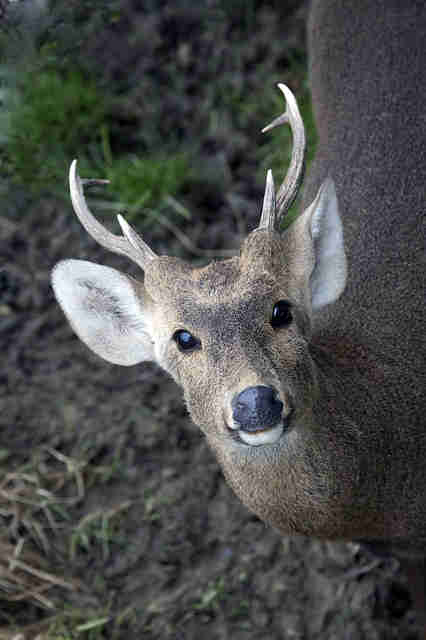
\includegraphics[scale=0.36]{../pictures/gazelle-compressed.jpg}\\
                    \caption{Komprimiert (1:5)}\label{fig:gazelle-compressed}
                \end{center}
            \end{figure}
        \end{multicols}

        \noindent
        Wenn wir viele der Koeffizieten nicht benutzen und trotzdem versuchen die Datenpunkte wiederherzustellen, kriegen wir lediglich eine Annäherung, wie man in Abbildung \ref{fig:gazelle-compressed} sieht. Sie ist meistens aber so gut genug, sodass wir keinen Unterschied merken. Eine sehr ähnliche Kompressionsmethode wird bei dem Bildformat JPEG \cite{jpeg} oder dem Videoformat MPEG \cite{mitchell1997mpeg} benutzt.

        \subsection{Kodierung des Suchraums}

            Diese Technik wenden wir nun auf die Gewichte von unserem neuronalen Netz an. Dafür beschränken wir den Suchraum auf eine kleine Anzahl der Koeffizienten und benutzen die inverse Kosinustransformation, um aus ihnen die nötige Anzahl von Gewichten zu erstellen. In Abbildung \ref{fig:dct-pre} und \ref{fig:dct-after} sieht man eine Anwendung auf 100 Gewichte, die ein Kompressionsverhältnis von 1:2 haben. Das bedeutet, dass wir den Suchraum mit dem in \ref{fig:dct-after} sichtbaren Genauigkeitsverlust halbiert haben.\\

            \noindent
            Bei größeren Verhältnissen bemerken wir eine starke örtliche Korrelation (\ref{fig:dct-my-case}) zwischen den benachbarten Zahlen und diese Eigenschaft passt zu der Annahme dass sich Gewichte in neuronalen Netzen ähnlich verhalten. Eine ausführlichere Erklärung findet sich im Ursprungspaper für die Anwendung in der Neuroevolution \cite{cosyne1}.
            \begin{multicols}{2}
                \begin{figure}[H]
                    \begin{center}
                        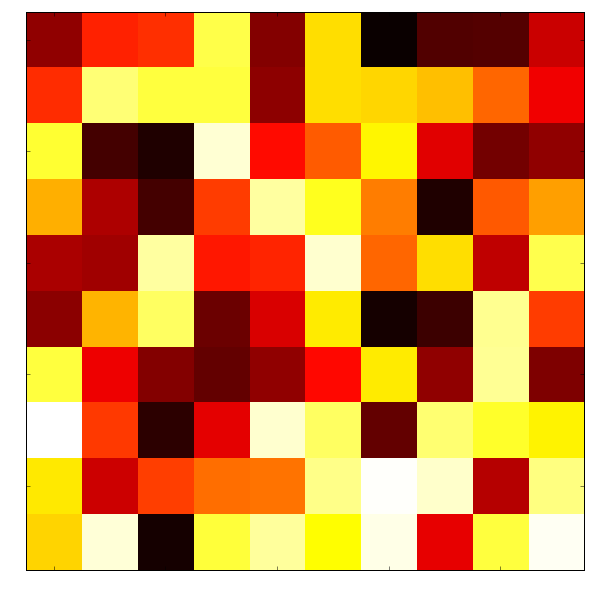
\includegraphics[scale=0.2]{../pictures/DCT-pre.png}\\
                        \caption{Unkomprimiert}\label{fig:dct-pre}
                    \end{center}
                \end{figure}
                \par
                \begin{figure}[H]
                    \begin{center}
                        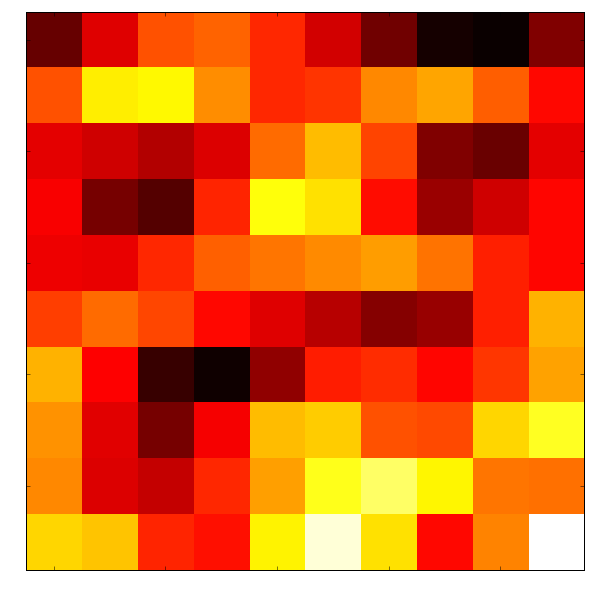
\includegraphics[scale=0.2]{../pictures/DCT-after.png}\\
                        \caption{Komprimiert (1:2)}\label{fig:dct-after}
                    \end{center}
                \end{figure}
            \end{multicols}

    \section{Cooperative Synapse Neuroevolution} \label{cosyne-definition}
        Nachdem wir den Zustandsraum komprimiert haben, sodass ein genetischer Algorithmus ihn in absehbarer Zeit entwickeln und ein neuronales Netz befüllt werden kann, erschließt sich die Verküpfung zu einem mächtigen Werkzeug das viele interessante Eigenschaften besitzt. Dieser Algorithmus wird Kooperative Synapsen Neuroevolution (\textbf{Cooperative Synapse Neuroevolution}) \cite{cosyne2}, oder auch \textbf{CoSyNE} genannt.\\

        \noindent
        Er zeichnet sich speziell dadurch aus, dass er auf kontinuierlichen Zuständen und Aktionen funktioniert und spärliche Fitnessignale interpretieren kann. Das schafft er, indem er rekurrente Netze aufbaut und die genetische Suche mit aggressiver Mutation im Zustandsraum beschleunigt. Ein gutes Beispiel dafür ist das Rennspiel \textbf{TORCS} \cite{cosyne3}, wo der Algorithmus 993 Gewichte in 33 Koeffizienten kodiert \textit{(Faktor 1:30)} und lediglich durch die Bilddaten ähnlich gute Ergebnisse liefert wie die per Hand programmierten Agenten, die die Physik des Spieles kennen.\\

        \noindent
        Ein großer Nachteil von genetischen Algorithmen ist, dass sie oft bei lokalen Maxima feststecken bleiben und lange brauchen um aus diesem Tal rauszukommen. Um dieses Problem anzugehen, versucht man die Stellschrauben wie Mutationswahrscheinlichkeit oder Kinderanzahl per Hand zu verändern \cite{grefenstette86}. CoSyNE benutzt dafür eine eigene \textbf{genetische Methode}, um die Suche einfacher zu gestalten. Sie nennt sich Permutation und erzeugt innerhalb der gesamten Population Unterteilungen in kleinere Populationen die in einer \textbf{kooperativen und koevolutionären} Beziehung stehen.
% \newpage
        \subsection{Permutation}
            Der Permutationsschritt wird ganz am Ende von dem genetischen Algorithmus statt der Repopulation aufgerufen und vermischt jeden \colorbox{green!25}{Eigenschaftsraum} der Gesamtpopulation. 

            \begin{table}[H]
                \begin{center}
                \begin{tabular}{ |r|r|r|r|r| } 
                    \hline
                    Individuum & \cellcolor{green!25} Höchstgeschwindigkeit & \cellcolor{green!25} Beinlänge & \cellcolor{green!25} Gewicht & \cellcolor{green!25} Hornlänge \\ \hline
                    $1$        & $60\; \frac{km}{h}$   & $40\; cm$ & $50\; kg$ & $10\; cm$ \\ \hline
                    $2$        & $61\; \frac{km}{h}$   & $41\; cm$ & $51\; kg$ & $11\; cm$ \\ \hline
                    $3$        & $62\; \frac{km}{h}$   & $42\; cm$ & $52\; kg$ & $12\; cm$ \\ \hline
                    $4$        & $63\; \frac{km}{h}$   & $43\; cm$ & $53\; kg$ & $13\; cm$ \\ \hline
                    $5$        & $64\; \frac{km}{h}$   & $44\; cm$ & $54\; kg$ & $14\; cm$ \\ \hline
                    $6$        & $65\; \frac{km}{h}$   & $45\; cm$ & $55\; kg$ & $15\; cm$ \\ \hline
                \end{tabular}
                \end{center}
                \caption{Vor der Permutation \label{fig:pre-perm}}
            \end{table}

            \begin{table}[H]
                \begin{center}
                \begin{tabular}{ |r|r|r|r|r| } 
                    \hline
                    Individuum & \cellcolor{green!25} Höchstgeschwindigkeit & \cellcolor{green!25} Beinlänge & \cellcolor{green!25} Gewicht & \cellcolor{green!25} Hornlänge \\ \hline
                    $1$        & \cellcolor{blue!45} $61\; \frac{km}{h}$   & \cellcolor{yellow!25} $43\; cm$ & \cellcolor{red!15} $54\; kg$ & \cellcolor{violet!45} $12\; cm$ \\ \hline
                    $2$        & \cellcolor{blue!45} $60\; \frac{km}{h}$   & \cellcolor{yellow!45} $44\; cm$ &                    $51\; kg$ & \cellcolor{violet!25} $14\; cm$ \\ \hline
                    $3$        & \cellcolor{blue!15} $64\; \frac{km}{h}$   & \cellcolor{yellow!65} $45\; cm$ & \cellcolor{red!35} $53\; kg$ & \cellcolor{violet!45} $10\; cm$ \\ \hline
                    $4$        &                     $63\; \frac{km}{h}$   & \cellcolor{yellow!25} $40\; cm$ & \cellcolor{red!35} $52\; kg$ & $13\; cm$ \\ \hline
                    $5$        & \cellcolor{blue!15} $62\; \frac{km}{h}$   & \cellcolor{yellow!45} $41\; cm$ &                    $54\; kg$ & \cellcolor{violet!25} $11\; cm$ \\ \hline
                    $6$        &                     $65\; \frac{km}{h}$   & \cellcolor{yellow!65} $42\; cm$ & \cellcolor{red!15} $50\; kg$ & $15\; cm$ \\ \hline
                \end{tabular}
                \end{center}
                \caption{Nach der Permutation \label{fig:pre-perm}}
            \end{table}

            \noindent
            Wenn wir uns die Population als zweidimensionale Liste vorstellen, wo jedes Indviduum eine eigene Liste mit seinen spezifischen Eigenschaften ist, können wir die Population transponieren, wobei nun jede Eigenschaft eine eigene Liste ist, diese zufällig vermischen und wieder zurück transponieren um die neuen Individuen zu bekommen. Der folgende Pythoncode veranschaulicht das Prinzip unter Verwendung der \textit{numpy} Bibliothek.

            \begin{mdframed}
            \begin{minted}[escapeinside=||, linenos]{python}
import numpy as np

i_1 = [1,10,100,1000] # Individuum 1-5
i_2 = [2,20,200,2000]
i_3 = [3,30,300,3000]
i_4 = [4,40,400,4000]
i_5 = [5,50,500,5000]

population = np.array([i_1, i_2, i_3, i_4, i_5])
eigenschaftsraum = np.transpose(population)
  
for eig in eigenschaftsraum:
    np.random.shuffle(eig)

population = np.transpose(eigenschaftsraum)

print population
> [[   2   40  500 5000]
   [   1   50  200 1000]
   [   4   10  300 3000]
   [   3   30  100 2000]
   [   5   20  400 4000]]

            \end{minted}
            \end{mdframed}
            \noindent
            Man erkennt leicht, dass keine der ursprünglichen Individuen erhalten bleiben und wir vollkommen neue bekommen. Der Sinn hinter dem Vermischen in der Eigenschaftsebene basiert auf der \textbf{Verknüpfungung mit der Kreuzungsmethode}. Wenn wir zwei Individuen kreuzen, werden ihre Kinder die gesamte Information von ihren Eltern in der Population übernehmen. Da CoSyNE den Repopulationsschritt nicht ausführt, dafür aber alle restlichen Individuen wegwirft, werden nur die Eigenschaften der Kinder übrig bleiben.\\

            \noindent
            Das führt zur Homogenität in den einzelnen Eigenschaften, die zum Beispiel dafür verantworlich ist, dass alle Individuen gleich große Hörner haben. Wenn nun innerhalb der Hornlänge zufällig gemischt wird, bleibt alles gleich, da die gesamte Liste aus dem gleichen Element besteht. \\

            \noindent
            Die Annahme von CoSyNE ist dass die Lösung für das Problem in der Kombination von den Eigenschaften von allen Individuen liegt, die wir am Anfang erstellen. Durch das aggressive Aussortieren durchsuchen wir den Raum aller Möglichkeiten schneller und darin liegt der größte Vorteil von diesem Algorithmus. Dieser Mechanismus wird als \textbf{kooperative Koevolution} im Eigenschaftsraum interpretiert, da wir jede Eigenschaft als Population betrachten und darin eine genetische Suche abhängig voneinander vollziehen \cite{cosyne2}. \\

            \noindent
            Wenn diese Annahme nicht stimmt und die Lösung nicht in einem Subset von allen Eigenschaften liegt, hat CoSyNE leider nur die Möglichkeit durch Mutation zum Ziel zu kommen. Deshalb wird dieser Parameter oft hoch gewählt \cite{cosyne1}\cite{cosyne2}\cite{cosyne3}.



\newpage
    \section{Cross Entropy Method} \label{cross-entropy-definition}
        Eine andere Möglichkeit die Individuen in dem GA zu kodieren stellt die \textbf{Cross Entropy Method} dar. Das ist ein Algorithmus der oft als Vergleichskriterium verwendet wird, da er oft zu suboptimalen Strategien konvergiert \cite{cem}. Die Anwendung in unserem neuroevolutionären Schema basiert darauf, dass wir Individuen nicht als Ansammlung von Zahlen zu speichern, sondern jede Eigenschaft als Normalverteilung dargestellt wird. Diese Abläufe illustrieren wir anhand der Erklärung für eine Normalverteilung \cite{ml-script}.

        \subsection{Normalverteilung}

            Eine Normalverteilung ist eine sehr bekannte stetige Wahrscheinlichkeitsverteilung. Ihre Wahrscheinlichkeitsdichtefunktion wird oft Gauß-Kurve oder Glockenkurve genannt und findet Anwendung in verschiedensten Anwendungsgebieten, weil sie natürliche Vorgänge exakt oder ähnlich genug modelliert. Bekannte Beispiele dafür sind die Streuung von Messfehlern oder die irreguläre Bewegung von Partikeln in einer Flüssigkeit (\textbf{Brownsche Bewegung}) \cite{Hida1980}.\\[2mm]
            \noindent
            Die Wahrscheinlichkeitsdichtefunktion der Normalverteilung ist von zwei Parametern abhängig, dem Durchschnitt und der Standardabweichung:
            \begin{figure}[H]
                \begin{mdframed}
                    \noindent
                    Sei $\mu$ der Durchschnitt,\\
                    \hspace*{4.5mm}    $\sigma$ die Standardabweichung, dann ist\\[4mm]
                    \hspace*{50mm} \Resize{6cm}{$\mathcal{N}(x\;|\;\mu, \sigma^2) = \frac{1}{\sqrt{2\pi\sigma^2}} \cdot e^{-\frac{(x - \mu)^2}{2\sigma^2}} $} \\[4mm]
                    \hspace*{4.5mm} die Wahrscheinlichkeitsdichtefunktion der Normalverteilung.
                \end{mdframed}
                \formforfigure
                \caption{\label{norm-dist-pdf-formel} Definition der Wahrscheinlichkeitsdichtefunktion der Normalverteilung}
            \end{figure}

            \begin{figure}[H]
                    \begin{center}
                        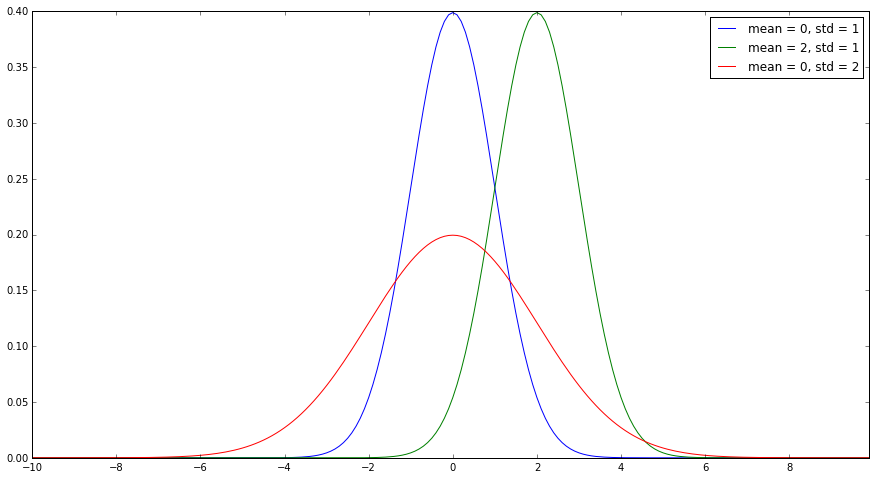
\includegraphics[scale=0.38]{../pictures/diagrams/normal-dist-example.png}\\
                        \caption{Dichtefunktionen von Normalverteilungen}\label{fig:norm-dist-pdf}
                    \end{center}
            \end{figure}

            \noindent
            Die Abbildung \ref{fig:norm-dist-pdf} zeigt beispielhafte Ausprägungen der Dichtefunktion, an denen man erkennen kann, dass die Standardabweichung für die Amplitute und der Durchschnitt für die Phase verantwortlich ist. Um die Wahrscheinlichkeit zu berechnen, dass eine zufällige Variable $\mathcal{X}$  mit den Grenzen $a \leq \mathcal{X} \leq b$ eintritt ist das Integral zwischen den Grenzen der Dichtefunktion:
            \begin{align}
                P(a \leq \mathcal{X} \leq b) = \int_a^{b} \; \mathcal{N} (\mu, \sigma^2)
            \end{align}

%            \begin{figure}[H]
%                \begin{mdframed}
%                    \hspace*{40mm} \Resize{6cm}{$P(a \leq \mathcal{X} \leq b) = \int_a^{b} \; \mathcal{N} (\mu, \sigma^2)$}
%                \end{mdframed}
%                \caption{Wahrscheinlichkeit der Ausprägung $a \leq \mathcal{X} \leq b$}
%            \end{figure}

            \noindent
            Diese Formel veranschaulichen wir an dem Beispiel von Regenfall pro Quadratmeter in Abbildung \ref{fig:rainfall-pdf}.

            \begin{figure}[H]
                    \begin{center}
                        \hspace{-1cm}
                        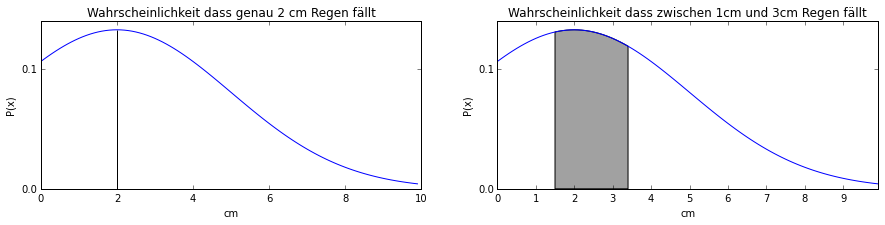
\includegraphics[scale=0.6]{../pictures/diagrams/rainfall-pdf.png}\\
                        \caption{Beispielhafte Dichtefunktion für Regenfall pro $m^{2}$}\label{fig:rainfall-pdf}
                    \end{center}
            \end{figure}
            \noindent
            Die Wahrscheinlichkeit, dass pro Quadratmeter \textit{genau} $2\;cm$ Regenwasser fällt ist extrem gering, weil nicht ein Yoctometer ($10^{-24})$ mehr oder weniger fallen darf. Wenn wir diese zufällige Ausprägung jedoch als Grenzen definieren, dann steigt die Wahrscheinlichkeit. Die Wahrscheinlichkeit dass zwischen $1\;cm$ und $3\;cm$ Regenwasser fällt ist eine viel wertvollere Aussage und ist als Integral zwischen den Grenzen der Dichtefunktion definiert.\\

            \subsection{Kodierung durch Normalverteilungen}

            \begin{figure}[H]
                    \begin{center}
                        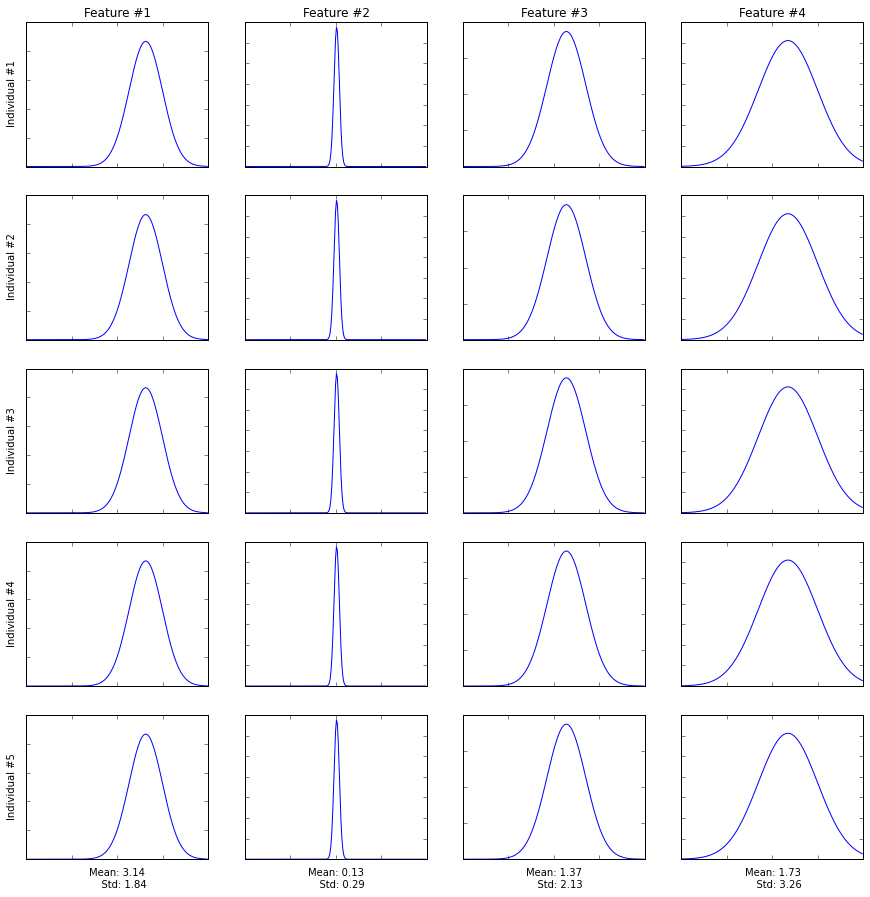
\includegraphics[scale=0.47]{../pictures/diagrams/cross-entropy-visualization-ga.png}\\
                        \caption{Kodierung der Eigenschaften durch Normalverteilungen}\label{fig:norm-dist-encoding}
                    \end{center}
            \end{figure}

            Stellen wir nun die Kodierung der Eigenschaften von jedem Individuum als Normalverteilung dar. Das bedeutet wir haben für jede Eigenschaft, zum Beispiel \textit{Hornlänge}, einen Durchschnitt und eine Standartabweichung. Die Abbilung (\ref{fig:norm-dist-encoding}) zeigt dies beispielhaft für fünf Individuen mit jeweils 4 Eigenschaften dar.\\[3mm]

            \newpage
            \noindent
            Wenn wir Individuen erstellen wollen, müssen wir aus jeder Normalverteilung eine Stichprobe nehmen (samplen), die wir als Punkte entlang der Graphen in \ref{fig:norm-dist-encoding} eingezeichnet haben.  Die Kreuzung und Mutation fallen aus, dafür berechnen wir nach jeder Simulation pro Eigenschaft neue Durchschnitte und Standartabweichungen aus den besten Individuen. Damit versuchen wir die Suche auf den vielversprechendsten Raum einzugrenzen.\\

            \noindent
            Der Ablauf der Cross Entropy Method sieht daher folgendermaßen aus \cite{cem-blog}:\\

                \begin{mdframed}
                    Sei $d$ die Anzahl der Eigenschaften,\\
                    \hspace*{5mm} $n$ die Anzahl der Individuen,\\
                    \hspace*{5mm} $\mu$, $\sigma$ jeweils ein Vektor der Form $\mathbb{R}^{d}$,\\
                    \hspace*{5mm} dann führen wir pro Iteration die folgenden Schritte durch: \\

                    \hspace*{8mm} 1. Wir nehmen $n$ Stichproben $\theta_i$ aus $\mathcal{N}(\mu, \sigma^{2})$ \\
                    \hspace*{12mm} 2. Evaluiere $\theta_i, i \in [1..n]$ in der Simulation\\
                    \hspace*{12mm} 3. Wähle die besten $p\%$ Prozent der Stichproben, wir nennen sie Eliteset\\
                    \hspace*{12mm} 4. Berechne aus den dem Eliteset neue $\mu$ und $\sigma$
                \end{mdframed}
            \hfill \\
            Eine viel detaillierte Erklärung zu diesem Thema findet sich am Beispiel von Tetris im dem Paper von István Szita \cite{cem}.
